\title{Study Guide for Midterm 3 for Algebra-Based Physics: Electricity and Magnetism}
\author{Dr. Jordan Hanson - Whittier College Dept. of Physics and Astronomy}
\date{\today}
\documentclass[10pt]{article}
\usepackage[a4paper, total={18cm, 27cm}]{geometry}
\usepackage{outlines}
\usepackage{graphicx}
\usepackage{amsmath}
\begin{document}
\maketitle

\section{Equations and constants}

\begin{enumerate}
\item Kirchhoff's Rules: 1) $I_{in} + I_{out} = 0$ (Junction Rule) 2) $\sum_{loop} V_i = 0$ (Loop Rule)
\item Power from current and voltage: $P = iV$
\item Power from currenta and resistance: $P = I^2 R$
\item Definition of magnetic flux: $\phi = \vec{B} \cdot \vec{A}$.  The units are T m$^2$, which is called a Weber, or Wb.
\item Faraday's Law: $emf = -N \frac{\Delta \phi}{\Delta t}$
\item Faraday's Law using \textbf{Inductance}, M: $emf = -M \Delta I / \Delta t$.
\item Magnetic permeability: $\mu_0 = 4\pi \times 10^{-7}$ T m A$^{-1}$
\item Units of inductance: V s A$^{-1}$, which is called a Henry, or H.
\end{enumerate}

\section{Exercises}

\begin{enumerate}
\item \textbf{Review Problem (similar exercise on the final)}
\begin{enumerate}
\item 
\begin{figure}[ht]
\centering
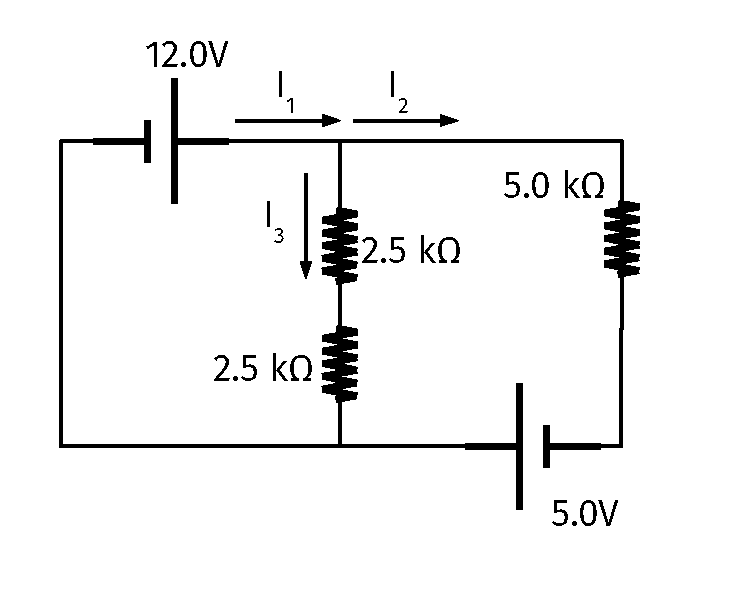
\includegraphics[width=0.3\textwidth]{iV.pdf}
\caption{\label{fig:circuit1} A circuit with three resistors.}
\end{figure}
Solve for the currents $I_1$-$I_3$ in Fig. \ref{fig:circuit1}. \\ \\ $I_3 = 12/5$ mA, $I_2 = 17/5$ mA, and $I_1 = 29/5$ mA. \\ \\
\item What is the power consumed by each resistor in Fig. \ref{fig:circuit1}? \\ \\ Two of the resistors (the ones with 2.5 k$\Omega$) each consume $P = IV = I_3 \times V_1 = 2.5 \times 10^{-3} \times 12.0$ W which is 30 mW.  The other resistor consumes $P = I^2 R = I_2^2 \times 5.0 $k $\Omega$, so $(17/5 \times 10^{-3})^2 5.0 \times 10^3 = 57.8$ mW.
\end{enumerate} \clearpage
\item \textbf{Chapter 23: Magnetic Induction, Faraday's Law, and AC power}
\begin{enumerate}
\item
\begin{figure}
\centering
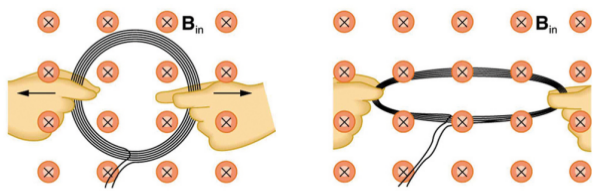
\includegraphics[width=0.4\textwidth]{flux1.png}
\caption{\label{fig:flux1} (Left) A magnetic field passes through loops of wire.  (Right) The loops are stretched, reducing the area.}
\end{figure}
In Fig. \ref{fig:flux1} (left) a uniform magnetic field passes through loops of wire.  In Fig. \ref{fig:flux1} (right) the \textbf{area} of the loops is reduced by stretching the loops.  Which of the following is true?
\begin{itemize}
\item A: No current flows through the wires.
\item B: Current does flow through the wires, but there is no induced emf in the wires.
\item C: Current flows through the wires, because the induced emf is caused by a change in electric flux.
\item D: Current flows through the wires, because the induced emf is caused by a change in magnetic flux.
\end{itemize}
(\textit{The answer is D. Magnetic flux $\phi = \vec{B} \cdot \vec{A} = BA$ in this case.  If the area changes, so does the flux.} \\ \\
\item Consider again the system in Fig. \ref{fig:flux1}.  The initial area is $A_i = 0.02$ m$^2$, the final area is one-half, or $A_f = 0.01$ m$^2$, and the transition from $A_i$ to $A_f$ takes 0.1 seconds.  The B-field strength is 0.1 T.  What is $\Delta \phi / \Delta t$? \\ \\
The change in flux is $\Delta \phi = B\Delta A$, because the B-field is not changing.  Thus, $\phi_f = BA_f$ and $\phi_i = BA_i$.  Subtracting, we get the change in flux: $\Delta \phi = B(A_f - A_i) = 0.1\times (0.02 - 0.01) = 0.1 \times 0.01 = 10^{-3}$ Wb.  That makes $\Delta \phi/\Delta t = 10^{-3}/0.1 = 10^{-2}$ Wb/s, or $10^{-2}$ V (10 mV). \\ \\
\item Continuing with Fig. \ref{fig:flux1}, if $\Delta \phi / \Delta t$ gives 10 mV, and the coil of wire has 100 turns, what is the induced emf in the coil? \\ \\ Apply Faraday's Law: $-N\Delta \phi /\Delta t = -100 * 10$ mV, or $-1.0$ V. \\ \\
\item
\begin{figure}
\centering
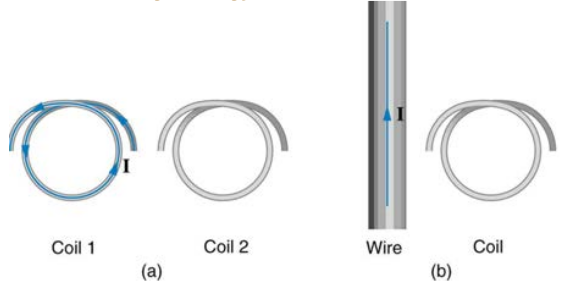
\includegraphics[width=0.4\textwidth]{flux2.png}
\caption{\label{fig:flux2} (a) The coils lie in the same plane. (b) The wire is in the plane of the coil.}
\end{figure}
Consider Fig. \ref{fig:flux2} (left).  In which direction is the current in the right-hand coil induced, if the current in the left-hand coil (a) increases?  (b) decreases? \\ \\
(a) If the counter-clockwise current on the left \textit{increases}, the corresponding flux \textit{into the page} in the right-hand coil  will increase.  Therefore, the right-hand coil will resist the change.  That means that the B-field generated will have to be \textit{out of the page} and therefore we get a \textbf{counter-clockwise} current.  (b) The exact opposite will happen if the current at left decreases, so we get a \textbf{clockwise} current. \\ \\
\item Assume that the current in the wire in Fig. \ref{fig:flux2} (right) is not changing.  (a) Is there any induced emf in the coil at right? (b) Suppose the current changes at a rate of 25.0 A/s, and the mutual inductance $M$ in the system is 0.1 mH.  What is the induced emf in the coil? \\ \\
(a) No - only if the current changes will there be any induced emf. (b) Applying Faraday's law with inductance, we have $emf = -M\Delta I/\Delta t = 0.1 \times 10^{-3} \times 25 = 2.5 \times 10^{-3} = 2.5$ mV.
\end{enumerate}
\end{enumerate}
\end{document}